\section{Risoluzione di problemi con la ricerca}
    Talvolta, scegliere un'azione in base a un obiettivo è semplice, quando quest'utlimo può essere raggiunto in un solo passo. Tuttavia non sempre è così, e l'agente potrebbe aver bisogno di percorrere un "cammino" che porta al risultato desiderato. Questi agenti sono più "flessibili" di quelli basati su modello.
    
    \paragraph{Rappresentazione atomica}
        In una rappresentazione atomica, uno stato è un elemento non divisibile, ossia astratto, che non ha una struttura interna. Gli algoritmi alla base di ricerca e giochi prendono in considerazione rappresentazioni atomiche del mondo.
        
    \subsection{Agenti risolutori di problemi}
        Gli agenti risolutori di problemi sono un particolare tipo di agenti basati su obiettivi, i quali si pongono uno o più obiettivi da raggiungere, e pertanto utilizzano una rappresentazione atomica del mondo, i cui stati verranno usati per trovare una soluzione accettabile al problema trattato.
        
        Sappiamo per esempio che le opzioni che rendono impossibile per l'agente raggiungere il proprio obiettivo verranno scartati: è totalmente inutile esplorare quelle opzioni. Ciò riduce notevolmente lo spazio delle possibili soluzioni, velocizzando la ricerca. Nel caso in cui due obiettivi implichino l'uno il fallimento dell'altro l'agente \underline{non} si blocca, ma tenta comunque di ottenere una soluzione buona, o quantomeno accettabile.
        
        Un'altra cosa che l'agente potrebbe fare in un contesto multi-obiettivo è evitare azioni che ottimizzino un solo obiettivo, anche perché ciò potrebbe andare a discapito degli altri.
        
        \paragraph{Formulazione dell'obiettivo.} Questo è necessariamente il primo passo della risoluzione di un problema. L'obiettivo è rappresentato da un insieme ammissibile di stati del mondo. Più in dettaglio, è rappresentato da tutti e soli quegli stati in cui l'obiettivo è soddisfatto.
        
        \subsubsection{Granularità}
            Se l'agente considerasse azioni di livello "troppo basso" (granularità alta), si ritroverebbe bloccato, in quanto si perderebbe in molti "microobiettivi" molto specifici, mentre al contrario un grado di granularità troppo basso potrebbe rendere la formulazione del problema troppo generica.
            
            Come astraiamo gli stati, possiamo estrarre anche le azioni. Ovviamente anche qui andrebbe scelto un grado di astrazione adeguato.
            
            Come uno stato è in realtà un insieme di stati più dettagliati, un'azione è un insieme di azioni più dettagliate.
            
            Un'astrazione si ritiene \textbf{valida} se possiamo espandere ogni soluzione astratta in una soluzione del mondo più dettagliata.
            
            Un'astrazione si definisce \textbf{utile} se eseguire ogni azione nell'astrazione è più facile che eseguirla nel problema originale.
            
            Ciò è vero ed utile perché gli agenti hanno l'arduo compito di lavorare in un mondo complesso senza però lasciarsi soverchiare dalla complessità del mondo.
            
        \subsubsection{Grado di conoscenza dell'agente}
            Se l'agente si trova in un ambiente ignoto, è costretto ad andare a caso, analizzando le sue azioni future per guadagnare conoscenza sulla qualità degli stati attualmente sconosciuti.
            
            Per un ambiente osservabile (si pensi a una mappa geografica, per esempio), l'agente conosce sempre lo stato del mondo. Se l'ambiente è \textbf{osservabile}, \textbf{discreto}, \textbf{noto} e \textbf{deterministico}, la soluzione è rappresentata da una sequenza finita di azioni, ed è rappresentabile tramite l'esplorazione di un grafo.
            
    \subsection{La Ricerca}
        Il processo che cerca una sequenza di azioni che portano al raggiungimento dell'obiettivo è proprio detto \textbf{ricerca}. La progettazione di un agente risolutore di problemi consiste dunque in 3 fasi: \textbf{formulazione}, \textbf{ricerca}, \textbf{esecuzione}.
        
        Un agente di questo tipo deve essere sicuro di ciò che accade nel mondo in quanto sceglie la sequenza di azioni da intraprendere all'inizio, a "occhi chiusi", e poi la esegue. Nella teoria del controllo si parla di sistema a ciclo aperto, in quanto ignorando la sequenza di percezioni si interrompe il ciclo fra agente e ambiente.
        
    \subsection{Problemi ben definiti e soluzioni}
        Un problema può essere definito formalmente tramite 5 componenti:
        \begin{enumerate}
            \item Stato iniziale.
            \item Azioni: l'insieme di azioni attuabili dall'agente in un dato stato.
            \item Modello di transizione: descrive il risultato dell'esecuzione di ogni azione.
            \item Test obiettivo: è il test di terminazione dell'algoritmo.
            \item Costo di cammino: determina il costo dell'esecuzione di un'azione.
        \end{enumerate}
        
        \paragraph{Stato degli spazi.}
            \textit{Stato iniziale}, \textit{azioni} e \textit{modello di transizione} definiscono lo stato degli spazi del problema, ossia l'insieme di tutti gli stati raggiungibili a partire da quello iniziale tramite una qualunque sequenza di azioni. Questo può essere rappresentato come un grafo.
            
\section{Ricerca non informata}
    Questo tipo di algoritmi, insieme agli algoritmi di ricerca informata, rappresentano la base della ricerca.
    
    L'essenza del concetto di ricerca sta nell'approfondire una soluzione e mettere da parte le altre (questo nel contesto del cosiddetto albero di ricerca). Nel caso pessimo si tornerà indietro per prendere in considerazione altre soluzioni.
    
    \paragraph{Cammini ciclici e ridondanti.}
        Se nell'albero un cammino è ripetuto più volte, parliamo di cammino ciclico, mentre il caso dei cammini ridondanti è più generale e lo abbiamo nel momento in cui esistono due o più modi per passare da uno stato all'altro.
        
        Sappiamo che ogni arco ha costo non negativo, quindi un ciclo non sarà mai conveniente e posso tranquillamente eliminarlo. Un cammino ridondante invece potrebbe essere necessario, nonostante potrebbe aumentare significativamente la difficoltà del problema: si pensi per esempio ai problemi le cui azioni sono reversibili.
        
        Per evitare di incappare in cammini ciclici o ridondanti, è utile avere una struttura dati denominata \textbf{insieme esplorato} (o \textbf{lista chiusa}). In questo modo l'albero di ricerca costruito tramite la ricerca avrà al più una copia di ciascuno stato.
        
    \paragraph{Nodi foglia e frontiera.}
        I nodi che in un determinato momento della ricerca non hanno figli vengono detti nodi foglia. L'insieme di tutti i nodi foglia in un determinato momento viene detta \textbf{frontiera}. Di norma avere questa struttura è utile in quanto andiamo a caricare un nodo in memoria solo quando viene aggiunto alla frontiera; avere tutti i possibili stati in memoria sarebbe troppo dispendioso, e a volte impossibile.
        
        Espandere la frontiera "a caso" non è certamente un modo viabile di esplorare lo spazio degli stati. Definiamo la \textbf{strategia} come la politica che l'algoritmo adotta per espandere la frontiera.
        
    \paragraph{Strutture dati per algoritmi di ricerca.}
        Gli algoritmi di ricerca hanno bisogno di strutture dati per tenere traccia e favorire l'esplorazione dell'albero fino ad ora generato. Ogni nodo $n$ dell'albero disporrà di una struttura dati avente i seguenti quattro componenti:
        \begin{itemize}
            \item \texttt{n.stato}: Lo stato attuale a cui corrisponde il nodo.
            \item \texttt{n.padre}: Il nodo dell'albero che ha generato il nodo corrente.
            \item \texttt{n.azione}: L'azione applicata al padre per generare il nodo.
            \item \texttt{n.costo-cammino}: Il costo $g(n)$ del cammino che va dallo stato iniziale ad $n$.
        \end{itemize}
        
        Abbiamo inoltre vari tipi di liste (FIFO, LIFO e coda a priorità) che possono essere usate per implementare la frontiera e determinano il criterio dell'espansione della suddetta.
        
    \subsection{Valutare un algoritmo di ricerca}
        Un algoritmo di ricerca è definito in base a una \textbf{modalità di espansione dei nodi}, ossia scegliendo l'ordine in base a cui i nodi sono espansi.
        
        Tali strategie vengono valutate in base a quattro fattori:
        \begin{itemize}
            \item \textbf{Completezza}: L'algoritmo \textit{garantisce} di trovare una soluzione, se questa esiste?
            \item \textbf{Ottimalità}: La soluzione trovata è \textit{ottima}?
            \item \textbf{Complessità temporale}: \textit{Quanto tempo} impiega l'algoritmo per trovare una soluzione?
            \item \textbf{Complessità spaziale}: Di \textit{quanta memoria} ha bisogno l'algoritmo per trovare una soluzione?
        \end{itemize}
        
        Al contrario dell'informatica teorica, in cui la complessità spaziale e temporale sono espresse in termini di dimensioni del grafo, nell'intelligenza artificiale il grafo è implicitamente descritto dallo stato iniziale, dal modello di transizione e dalle azioni: è quindi spesso indefinito, e lo descriviamo in termini diversi da $\vert E \vert$ e $\vert V \vert$, e ossia:
        \begin{itemize}
            \item $b$, il fattore di ramificazione o branching factor.
            \item $d$, profondità della soluzione a costo minimo o depth.
            \item $m$, ossia massima profondità dello spazio degli stati.
        \end{itemize}
        
        \subsection{Strategie di ricerca non informata}
            
            Le strategie di \textbf{ricerca non informata} non dispongono di ulteriori informazioni sugli stati, sanno solo distinguere fra un nodo obiettivo e uno non obiettivo. Quindi la principale differenza fra le strategie sta nell'ordine in cui verranno espansi i nodi della frontiera. Vediamo alcuni di questi algoritmi.
            
            \paragraph{Ricerca in ampiezza.} Tutti i nodi di profondità $d$ vengono esplorati prima di passare a quelli di profondità $d+1$. Essendo una strategia di ricerca \textbf{sistematica}, troverà una soluzione. Questa tuttavia non sarà ottima, in quanto sarà quella che richiede l'esplorazione di meno nodi, ma non tiene conto in nessun modo del peso degli archi che collegano tali nodi.
            
            Dal punto di vista pratico questa strategia può essere implementata utilizzando una semplice coda FIFO per la frontiera. La complessità temporale sarà esponenziale, mentre quella spaziale sarà dominata dalla dimensione della frontiera.
            
            \paragraph{Ricerca a costo uniforme.} Piuttosto che espandere il nodo più vicino alla radice, questo tipo di ricerca espande il nodo con costo di cammino minore.
            
            È possibile realizzare questo tipo di ricerca memorizzando la frontiera come una coda a priorità ordinata secondo il costo di cammino $g$ - in cima ci saranno i nodi di costo minore.
            
            Altre due differenze implementative rispetto alla ricerca per ampiezza sono che il test obiettivo è applicato a un nodo appena è selezionato per l'espansione, e non quando viene generato per la prima volta, e che si aggiunge un test obiettivo nel caso in cui sia trovato un cammino migliore per raggiungere un nodo che attualmente è sulla frontiera.
            
            Questo algoritmo è sia completo che ottimo, tuttavia è molto poco efficiente.
            
            \paragraph{Ricerca in profondità.} In questa strategia di ricerca espandiamo il nodo più profondo. Questo tipo di ricerca usa una coda LIFO.
            
            Questo algoritmo potrebbe non terminare, per esempio nel caso di cicli o cammini ridondanti, quindi non è completo. Non è nemmeno ottimo, in quanto nulla ci dice che anche quando trova una soluzione sia quella ottima e anzi, sappiamo che ciò è poco probabile in quanto questa soluzione tenderà a essere lontana dalla radice.
            
            Ha una complessità spaziale più appetibile, ma la complessità temporale resta esponenziale.
            
            \paragraph{Ricerca in profondità limitata.} Possiamo imporre un limite alla profondità della ricerca dell'algoritmo precedente. In questo modo evitiamo il problema della non terminazione, ma introduciamo una nuova fonte di incompletezza. Potremmo trovare lo stato obiettivo, potremmo non trovare nessuna soluzione o raggiungere il limite stabilito senza aver trovato nessuna soluzione.
            
            Questo metodo di ricerca non è completo né ottimo, la sua complessità temporale è dominata dalla profondità massima stabilita, mentre quella spaziale è dell'ordine del valore di suddetto limite moltiplicato il branching factor, in quanto una volta che tutti i discendenti di un nodo sono stati esplorati completamente, esso può essere rimosso.
            
            \paragraph{Ricerca ad approfondimento iterativo.} Con questo tipo di ricerca il limite viene incrementato iterativamente fino a che un nodo obiettivo non viene trovato. Questo metodo è analogo alla ricerca in ampiezza, in quanto ogni livello viene esplorato prima di passare a una profondità maggiore.
            
            Abbiamo la completezza e, se il costo di cammino è una funzione monotona non decrescente, anche l'ottimalità. La complessità temporale è esponenziale ma quella spaziale è analoga alla ricerca in profondità limitata.
            
            \paragraph{Ricerca bidirezionale.} L'idea alla base è quella di effettuare due ricerche, una guidata dagli obiettivi e l'altra guidata dai dati. Una ricerca viene effettuata all'avanti a partire dallo stato iniziale, l'altra all'indietro dallo stato obiettivo. Se le frontiere delle due ricerche si intersecano, abbiamo trovato l'obiettivo.
            
            È tuttavia molto difficile definire e implementare una ricerca "all'indietro".
            
\section{Ricerca Informata}
    Gli algoritmi di ricerca informata sfruttano conoscenze specifiche del problema allo scopo di essere più efficienti.
    
    L'approccio generale viene chiamato di ricerca \textbf{best-first}: la sua implementazione è molto simile a quella dell'algoritmo di ricerca a costo uniforme, ma la coda a priorità è ordinata in base a una funzione di valutazione $f(n)$. Spesso questa funzione di valutazione esiste nella forma di una funzione euristica $h(n)$. Le euristiche sono spesso il modo migliore per aggiungere conoscenza in un algoritmo di ricerca.
    
    \subsection{Ricerca best-first greedy}
        Un algoritmo greedy espande il nodo più vicino all'obiettivo, con la speranza che iterando questo comportamento più volte si possa arrivare all'obiettivo in maniera efficiente.
        
        Questo avviene applicando come funzione di valutazione direttamente la funzione euristica.
        
        Questo tipo di algoritmi non sono \textbf{completi} né tantomeno \textbf{ottimi}: la loro incompletezza è data dal fatto che potrebbero trovarsi in un "vicolo cieco", portati lì perché la strada per arrivare a suddetto vicolo cieco è molto poco costosa. Per lo stesso motivo potrebbero incappare in cicli infiniti.
        
        Anche quando riescono a trovare una soluzione, sappiamo che avranno ignorato eventuali archi costosi, anche se seguiti da cammini molto poco costosi. È ragionevole pensare che un cammino di questo tipo potrebbe essere ottimo, ma l'algoritmo non lo saprà mai in quanto l'iniziale arco costoso sarà un deterrente per lui, e gli impedirà di intraprendere questo cammino potenzialmente ottimo.
        
        La \textbf{complessità temporale} sarà, nel caso pessimo $\mathcal{O}(b^m)$, con $m = $ massima profondità dello spazio di ricerca, ma potrebbe essere drasticamente migliorata da una buona euristica.
        
        La \textbf{complessità spaziale} sarà ancora uguale a $\mathcal{O}(b^m)$, in quanto l'algoritmo terrà in memoria tutti i nodi.
        
    \subsection{Ricerca A*}
        Abbiamo una leggera ma molto più efficace variazione del precedente algoritmo nella forma della \textbf{Ricerca A*}. Essa è la forma più diffusa di ricerca best-first, e la otteniamo combinando il costo per raggiungere il prossimo nodo, ossia $g(n)$, con il costo stimato da suddetto nodo all'obiettivo, ossia $h(n)$. In pratica, abbiamo $f(n) = g(n) + h(n)$, con $h(n) > 0$ e $h(goal) = 0$.
        
        Possiamo intuire che è possibile ricadere in un paio di casi particolari:
        \begin{itemize}
            \item Se $h(n) = 0$, allora $f(n) = g(n)$ e ricadiamo nel caso di una Ricerca Uniforme.
            \item Se invece $g(n) = 0$, allora $f(n) = h(n)$ e ricadiamo nel caso di una ricerca best-first greedy.
        \end{itemize}
        
        L'\textbf{ottimalità} di A* dipende da due fattori:
        \begin{itemize}
            \item Il primo è che $h(n)$ sia un'euristica ammissibile, ovvero che non sbagli mai per eccesso la stima del costo per arrivare all'obiettivo.
            \item La seconda è che $h(n)$ sia un'\textbf{euristica consistente}. Per ogni nodo $n$ e per ogni suo successore $n'$ generato da un'azione $a$, il costo stimato per raggiungere l'obiettivo partendo da $n$ non è superiore al costo di passo per arrivare a $n'$ sommato al costo stimato da $n'$ all'obiettivo.
        \end{itemize}
        
        \paragraph{Completezza:} L'algoritmo è completo se esiste un numero finito di nodi di costo minore o uguale a $C*$ (la soluzione ottima), una condizione vera se tutti i costi dei passi superano un valore finito $\varepsilon$ e se $b$ è finito.
        
        \paragraph{Complessità temporale:} L'algoritmo è ottimamente efficiente. A parità di euristica, nessun altro algoritmo espande meno nodi senza rinunciare all'ottimalità. L'algoritmo ha complessità $\mathcal{O}(b^\varepsilon)$, il che lo rende il più efficiente fra gli algoritmi best-first.
        
        \paragraph{Complessità spaziale:} L'algoritmo tiene in memoria tutti i nodi generati, quindi $\mathcal{O}(b^m)$.
        
    \subsection{Beam Search}
        Abbiamo fino ad ora migliorato la complessità temporale degli algoritmi, ignorando tuttavia quella spaziale. Possiamo lavorare su questo aspetto tramite la \textbf{Beam Search}. Questo tipo di ricerca è una variante della best-first che non tiene in memoria tutti i nodi generati, ma solo i $k$ più promettenti, con $k$ definito come \textit{ampiezza del raggio}. Possiamo definire questa ampiezza in base a un'euristica adeguata.
        
        Sebbene migliori di molto l'occupazione di memoria (la sua complessità spaziale è $\mathcal{O}(kd)$), l'algoritmo non è ottimo né completo.
        
    \subsection{Iterative Deepening A* (IDA*)}
        Questo tipo di ricerca applica il concetto di approfondimento iterativo al contesto della ricerca euristica. 
        
        La differenza principale fra l'approfondimento iterativo e la ricerca IDA* sta nel valore del taglio, che non è più basato sulla profondità ma sul costo $g$, ovvero su $g+h$.
        
        Ad ogni iterazione il nuovo valore di taglio è l'$f$-costo minimo tra quelli di tutti i nodi che hanno superato il valore di taglio nell'iterazione precedente.
        
        Essendo un'estensione di A* manteiene le proprietà di ottimalità e completezza, a patto che sussistano le condizioni di ammissibilità e consistenza dell'euristica.
        
        L'algoritmo mantiene le caratteristiche di complessità spaziale della ricerca iterativa, e dovrà mantenere in memoria solo un cammino dalla radice al nodo foglia, più i fratelli non espansi di ogni nodo del cammino. Una volta che tutti i discendenti di un nodo sono stati esplorati completamente, esso può essere rimosso dalla memoria. La complessità è dunque $\mathcal{O}(bd)$.
        
    \subsection{Ricerca best-first iterativa}
        Questa rappresenta una variante della ricerca best-first classica, ma utilizza uno spazio lineare.
        
        Ad ogni iterazione l'algoritmo tiene traccia del miglior percorso \textit{alternativo}. Invece di fare backtracking in caso di fallimento, interrompe l'esplorazione quando trova un nodo meno promettente.
        
        L'\textbf{ottimalità} si ottiene nel caso in cui l'euristica sia ammissibile. La \textbf{complessità spaziale} è invece di nuovo $\mathcal{O}(bd)$, mentre quella \textbf{temporale} è difficile da definire, siccome dipende dalla funzione euristica e dalla frequenza dei cambi di percorso, ma nel caso peggiore sarà esponenziale.
        
        \textbf{Il problema }\color{black}della RBFS, ma anche della ricerca IDA*, sta nel fatto che usano \textbf{troppa poca memoria}. Hanno una complessità spaziale lineare, ma anche se avessero a disposizione più memoria non saprebbero usarla. Il risultato è che dimenticano la maggior parte delle cose che fanno, rischiando così di ripetere più e più volte gli stessi percorsi.
        
    \subsection{Simplified Memory Bounded A* (SMA*)}
        L'idea è di usare al meglio la memoria disponibile. Molto semplicemente, SMA* procede come A* fino all'esaurimento della memoria disponibile.
        
        Quando esaurisce la memoria, l'algoritmo libera il nodo peggiore, tenendo tuttavia in memoria il suo genitore. Questo permette all'algoritmo di tenere traccia della radice di un sottoalbero dimenticato, e di conseguenza un'informazione ($h(padre(n))$) sul cammino migliore di quel sottoalbero. Questo sottoalbero verrà rigenerato se e quando tutti gli altri cammini si saranno rivelati peggiori.
        
        SMA* è \textbf{completo} se esiste una soluzione raggiungibile, ossia se la profondità della soluzione è inferiore alla dimensione della memoria espressa in nodi.
        
        È inoltre \textbf{ottimale} se esiste una soluzione ottima raggiungibile.
        
        La \textbf{complessità temporale} potrebbe tuttavia esplodere nel caso di problemi difficili, rendendo il problema intrattabile.
        
    \subsection{La lezione da apprendere}
        Anche restando in un contesto di complessità esponenziale, si può migliorare di molto l'efficienza, o aumentare la porzione di spazio degli stati esplorata, tramite una buona euristica.
        
        Potrei dovermi anche trovare a "inventare" o modificare delle euristiche, per esempio combinandole, prendendone il massimo, definendo una loro priorità, rilassando i vincoli, etc.

\newpage
\section{Algoritmi di Ricerca Locale}
    Fino ad ora abbiamo visto algoritmi che esplorano sistematicamente lo spazio degli stati e, per come li abbiamo definiti, restituiscono la sequenza di passi da eseguire per raggiungere la soluzione.
    
    Tuttavia, facciamo un passo verso formulazioni più realistiche di problemi: in contesti reali spesso non ci interessa della sequenza di passi intrapresa per raggiungere un obiettivo; \textbf{la soluzione è lo stato obiettivo stesso}. Si pensi per esempio al problema delle 8 regine, alla disposizione di tavoli in un ristorante, eccetera.
    
    In questo contesto lo spazio degli stati è dato dall'insieme delle configurazioni "complete", ovvero quelle che portano a uno stato obiettivo. Lo scopo in questo caso sarà di tenere conto dello stato corrente con lo scopo di migliorarlo. La soluzione trovata potrebbe essere sub-ottimale, ma sicuramente ne gioverà l'utilizzo di memoria e le prestazioni.
    
    \paragraph{La funzione obiettivo.}
        Gli algoritmi di ricerca locale, spesso e volentieri, non disporranno di un test obiettivo (sia per la sua poca utilità in questo contesto, sia perché spesso è difficile da definire), ma di una funzione obiettivo, che indica quanto la ricerca sta migliorando da un'iterazione all'altra.
        
        Da qui definiamo la \textbf{struttura dei vicini}, ossia un sottoinsieme dello spazio degli stati relativo allo stato corrente, e in particolare quegli stati che sono immediatamente raggiungibili dallo stato corrente.
        
        È da notare che non necessariamente la soluzione raggiunta sarà globalmente ottima, ma sicuramente sarà ottima rispetto al suo circondario, ossia rispetto alle circostanze correnti.
        
    \paragraph{Lo spazio degli stati.} È utile visualizzare lo spazio degli stati come un grafo, e non come un albero, dove  sull'asse verticale abbiamo il valore della funzione obiettivo.
    
    \begin{figure}[h]
        \centering
        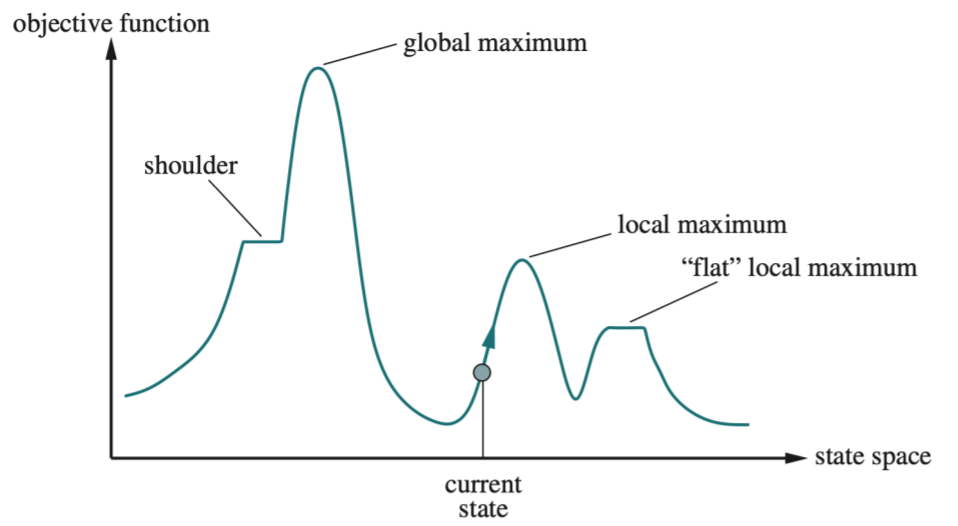
\includegraphics[width=0.8\textwidth]{img/img2.png}
        \caption{Lo spazio degli stati visualizzato come un grafo.}
        \label{fig:img2}
    \end{figure}
    
    Come possiamo vedere ci sono una serie di situazioni da tenere in conto: potremmo trovarci bloccati su un plateau, come su una spalla, o ancora potremmo concludere l'esecuzione di un algoritmo dopo aver trovato solo un massimo locale. Per ognuno di questi problemi ci sono una serie di soluzioni che vedremo in seguito. 
    
    \paragraph{Ottimi locali e globali.} Per ottimo locale intendiamo uno stato che ha una funzione obiettivo con un valore migliore rispetto al suo vicinato. Più è largo il vicinato e più è probabile che questo ottimo locale sia anche un ottimo globale. Infatti, per ottimo globale intendiamo quello stato il cui valore della funzione di valutazione è migliore di quello di qualunque altro stato. 
    
    \subsection{L'algoritmo Hill-Climbing}
        Questo è l'algoritmo più semplice fra quelli di ricerca locale e ha l'obiettivo di "scalare" lo spazio di ricerca finché non trova un ottimo, sia esso locale o globale.
        
        Quando il nodo corrente è migliore di tutti i suoi vicini, l'algoritmo si ferma. Questo rende l'algoritmo molto efficiente dal punto di vista della memoria, ma lo rende anche particolarmente vulnerabile a \textit{ridges}, \textit{plateaus} e soprattutto ottimi locali. Questo rende l'algoritmo assolutamente non ottimale, ma la sua altissima efficienza può renderlo comunque desiderabile in contesti realistici.
        
        \paragraph{Possibili miglioramenti.} Potrebbe valere la pena di eseguire mosse laterali in presenza di un plateau, nella speranza che sia una spalla. Tuttavia questo non è vero in generale. La soluzione è stabilire un numero massimo di mosse laterali dopo le quali si stabilisce il plateau come ottimo locale. 
        
        \paragraph{Varianti dell'algoritmo Hill-Climbing.} Alcune varianti includono:
        \begin{itemize}
            \item \textbf{Hill-Climbing stocastico:} Sceglie a caso fra le mosse che offrono un miglioramento, anziché scegliere quella che offre il miglioramento maggiore. Questo permette all'algoritmo di esplorare lo spazio degli stati in maniera spesso più completa.
            \item \textbf{Hill-Climbing con prima scelta:} Può generare mosse a caso fino a trovarne una migliore dello stato corrente. Questo è utile nel caso in cui ogni stato abbia moltissimi successori.
            \item \textbf{Hill-Climbing con riavvio casuale:} Può ricominciare da un punto casuale dello spazio degli stati. È da notare che generare un punto casuale dello spazio degli stati è di per sé un problema difficile.
        \end{itemize}
            
    \subsection{Algoritmo Simulated Annealing}
        Un algoritmo che non scende mai "a valle" ma che tende sempre e comunque a salire potrebbe restare bloccato con grande facilità in ottimi locali. Al contrario, una ricerca casuale è completa ma estremamente inefficiente.
        
        L'algoritmo di \textbf{Simulated Annealing} si porpone di combinare le due cose. In metallurgia l'annealing è il processo di riscaldare molto un metallo per poi raffreddarlo gradualmente, in maniera da permettergli di cristallizzare in uno stato a bassa energia. Il corrispettivo nel contesto della ricerca è di "scuotere" molto la ricerca in una fase iniziale, così da variare molto il panorama degli stati, per poi stabilizzarsi e concentrarsi su un punto specifico del panorama, cercando un ottimo in quel contesto.
        
        Ciò che succede in pratica è che mosse "cattive" verranno accettate più facilmente all'inizio ma diventeranno sempre meno probabili man mano che la temperatura si abbassa. Più si abbassa la temperatura, più probabilmente l'algoritmo troverà un ottimo globale, con probabilità tendente a 1.
        
    \subsection{Algoritmo Local Beam}
        L'algoritmo Local Beam è una versione meno estrema della Beam Search vista in precedenza. Anziché tenere in memoria un solo stato, ne tiene in memoria $k$. Inizia generando casualmente $k$ stati e generandone tutti i successori. Se fra questi c'è l'ottimo concludi la ricerca, altrimenti prendi i $k$ migliori e ricomincia. Potrebbe sembrare simile all'algoritmo hill-climbing con riavvio casuale, ma in questo caso c'è dell'informazione che viene scambiata fra i vari "thread". Il rischio è che gli stati potrebbero convergere troppo velocemente in una piccola regione dello spazio.
        
    \subsection{Local Beam Stocastica}
        Si basa sulla ricerca previamente vista. Tuttavia, anziché scegliere i $k$ migliori successori ne vengono scelti $k$ a caso, con l'accortezza di assegnare ai più promettenti una maggiore possibilità di essere scelti. Questo funge da base per gli algoritmi genetici.
       
\newpage
\section{Algoritmi Genetici}
    La teoria della \textbf{selezione naturale} proposta inizialmente da Charles Darwin è riassumibile in quattro punti cardine:
    \begin{itemize}
        \item \textbf{Variation:} Gli individui di una popolazione differiscono nel patrimonio genetico, e ciò implica molte differenze fisiche.
        \item \textbf{Inheritance:} Gli individui si riproducono e trasmettono parte del loro patrimonio genetico alla prole.
        \item \textbf{Selection (and adaptation):} Alcuni individui possiedono tratti ereditari che li renderanno più adatti a sopravvivere e riprodursi; questi tratti saranno dunque presenti in buona parte della popolazione.
        \item \textbf{Time:} A lungo andare la selezione può comportare la nascita di nuove specie (\textit{speciazione}).
    \end{itemize}
    
    \subsection{Teoria dell'Evoluzione e Ottimizzazione}
        Ovviamente il nostro scopo non è studiare la teoria dell'evoluzione, per quanto sia una delle teorie più potenti della storia, ma algoritmi di ricerca. Come possiamo dunque adattare i concetti previamente spiegati alla ricerca? Cosa intendiamo per generazioni, individui e selezione?
        
        Dobbiamo innanzitutto capire con cosa abbiamo a che fare. Supponiamo di avere una funzione matematica da ottimizzare. Abbiamo uno spazio di ricerca in cui lavorare, ottimi locali e globali e una funzione, detta funzione obiettivo, da poter testare. Alcuni tipi di ricerca ci permettono di raggiungere l'ottimo globale, ed essi sono detti ottimi, ma sicuramente non tutti ci permettono questo lusso. 
        
        Quando non è realistico pensare di trovare l'ottimo globale, dobbiamo accontentarci di \textbf{soluzioni approssimate}, ragionevolmente buone e non proibitive da trovare.
        
        Possiamo inoltre pensare, anziché pensare di partire da una singola soluzione e migliorarla iterativamente, di partire da diverse soluzioni e premiare quelle più promettenti. Questa idea è alla base della \textbf{ricerca globale}.
        
    \subsection{Algoritmi Genetici}
        Gli \textbf{algoritmi genetici} sono una sottocategoria degli algoritmi evolutivi, ossia algoritmi ispirati alla teoria dell'evoluzione, i quali sono a loro volta una sottocategoria degli algoritmi ispirati alla natura.
        
        Una delle prime definizioni di \textbf{algoritmi genetici} li identifica come meta-euristiche. Sono molto utilizzati proprio per la loro poca specificità e quindi possibilità di adattarsi a molti problemi e avere un grande numero di varianti che possono ospitare comodamente euristiche e adattamenti.
        
        Proviamo a darne una \textbf{definizione} abbastanza generica: un algoritmo genetico (GA) fa \textit{evolvere} una \textit{generazione} di individui iterativamente, producendo di volta in volta generazioni migliori, rispetto a una cosiddetta \textit{misura di fitness}, finché non si verifica un \textit{criterio di arresto}. La generazione di nuovi individui avviene tramite tre operatori di ricerca, quali \textbf{selezione}, \textbf{crossover} e \textbf{mutazione}.
        
        Goldberg identifica 4 \textbf{caratteristiche fondamentali} dei GA:
        \begin{itemize}
            \item \textbf{Encoding:} La maniera in cui viene codificato (rappresentato) un individuo.
            \item \textbf{Global Search:} Un GA usa un insieme di soluzioni candidate per esplorare più punti dello spazio di ricerca. Questo diminuisce le possibilità di bloccarsi in ottimi locali.
            \item \textbf{Blindness:} Un GA non ha bisogno di conoscere la funzione da ottimizzare, questa può essere accessibile in forma \textit{black-box}.
            \item \textbf{Probabilistic:} Un GA include elementi di casualità che guidano la ricerca pur non sfociando in un random search.
        \end{itemize}
        
        \subsection{Punti di forza.}
            I GA sono caratterizzati da molte componenti: codifica degli individui, funzione obiettivo, mutazioni, selezione, eccetera. La loro forza risiede proprio in questo: sono algoritmi abbastanza flessibili da poter adattare i problemi all'algoritmo anziché creare un algoritmo apposito per il problema. Il problema potrebbe avere molti aspetti difficili da affrontare, mentre una volta adattato al GA avrà una quantità discreta di parametri semplici.
            
            Tuttavia vale la pena far notare che la maggior difficoltà risiede in soli due aspetti.
        
            \subsubsection{Codifica degli individui.}
                La codifica di Holland prevede la codifica in stringhe binarie di dimensione finita, ma queste tendono a essere lunghe e talvolta difficili da trattare e interpretare. Possiamo dunque pensare di avvalerci di una serie di strutture dati da usare come codifica degli individui: vettori di numeri reali, vettori di interi, alberi, interi blocchi di codice, eccetera.
                
                Questo potrebbe, fra le altre cose, favorire molto il processo di crossover. Pensiamo di codificare due punti su un grafo come coordinate di interi. Possiamo pensare di prendere il punto intermedio fra di essi, cosa che risulterebbe sicuramente più difficile con stringhe binarie.
                
                Inoltre strutture dati alternative potrebbero darci implicitamente informazioni sul problema che stiamo affrontando. Pensiamo al problema delle 8 regine e di codificare le soluzioni come vettori di interi che vanno da 0 a 7, i quali rappresentano la posizione verticale di una regina sulla colonna corrispondente all'indice del vettore; questo ci dice implicitamente che non possiamo avere due regine sulla stessa colonna, cosa che sarebbe invece possibile codificando gli individui come 8 vettori binari lunghi 8 (in pratica dunque una matrice binaria 8x8), con 0 che rappresenta l'assenza di una regina sulla casella e 1 che ne rappresenta la presenza.
            
            
            \subsubsection{Funzione obiettivo.}
                Ricordiamo prima una importante distinzione. La \textbf{funzione obiettivo} è la funzione da ottimizzare, e modella il problema. La \textbf{funzione di valutazione} viene applicata a un individuo e ne calcola la qualità.
                
                Detto ciò, è bene notare che spesso le due cose coincidono, ossia viene utilizzata la funzione obiettivo come funzione di valutazione. Possiamo riservarci tuttavia il diritto di non applicare questa scelta nel caso in cui, per esempio, applicare la funzione obiettivo sia dispendioso.
                
                Spesso la \textbf{funzione obiettivo} non è definita intrinsecamente nel problema, ma siamo noi a doverla definire, cosa che ci lascia un certo grado di libertà ma anche una certa responsabilità. Se la nostra funzione obiettivo non è applicabile in tempi ragionevoli, possiamo definire una funzione di valutazione che approssima la funzione obiettivo.
                
            
            \subsubsection{Selezione}
                È ciò che permette agli individui migliori di una generazione di passare i loro geni alla prossima. Fornisce a un individuo un \textbf{punteggio di fitness} usando una \textbf{funzione di fitness}.
                
                Una funzione di tipo \textit{fitness proportionate} (basata sulla valutazione relativa di ciascun individuo rispetto agli altri) porta con sé alcuni rischi. Infatti si rischia, specialmente in popolazioni di piccola taglia, di favorire troppo individui con alto punteggio di fitness, che andranno a monopolizzare la popolazione. Ciò è una cosa negativa in quanto gli algoritmi genetici fanno della \textit{diversità} fra gli individui il loro punto di forza, usando individui apparentemente svantaggiosi per uscire da ottimi locali.
                
                In questo caso parliamo di \textbf{convergenza prematura}, che si osserva quando l'evoluzione smette di dare miglioramenti notevoli troppo presto. Le soluzioni a questo problema sono molteplici, e spesso si basano sul concetto di favorire individui forti senza tuttavia trascurare quelli deboli.
                
                Un altro concetto che appare nella fase di selezione è quello di \textbf{ricampionamento}. Un metodo di selezione con ricampionamento permette allo stesso individuo di essere selezionato più volte, e in questo caso è possibile avere una mating pool grande quanto la popolazione. Viceversa essa deve essere necessariamente più piccola nel caso di una selezione senza ricampionamento.
                
                \paragraph{Rango.} Possiamo per esempio definire il \textit{rango} come la posizione nell'ordinamento secondo il punteggio di fitness, e dare a un individuo una probabilità di essere selezionato relativa al suo rango. È applicabile anche con valutazioni negative, e compensa differenze di valutazioni troppo grandi fra i singoli individui.
                
                \paragraph{Tournament selection.} Un altro metodo di selezione è quello di formare un torneo di $K$ individui, con $1 < K < \vert P \vert$, e far passare il migliore. Si ripete il processo fino ad avere il numero di individui desiderato. Oltre a essere applicabile anche con valutazioni negative, non richiede nessun ordinamento.
                
                \paragraph{Elitismo.} Non di per sé un metodo di selezione, è piuttosto un metodo per evitare che vengano scartati individui molto buoni. Il concetto alla base è quello di far passare un tot$\%$ degli indiidui migliori, copiandoli direttamente alla prossima generazione. Canonicamente questo campione di individui, chiamato \textit{elite}, non dovrebbe partecipare né a crossover né alla selezione, ma nulla ci vieta di farlo lo stesso.
                
            \subsubsection{Crossover}
                L'operatore di \textbf{corssover} rappresenta il primo passo per l'esplorazione di parti dello spazio di ricerca previamente inesplorate.
                
                Questo operatore è particolarmente sensibile alla codifica degli individui, e deve essere \textbf{sensato}. Un esempio, che ha senso per stringhe di elementi, è il \textbf{single-point crossover}, in cui scegliamo un punto di crossover e prendiamo la porzione precedente al punto dal primo genitore e la porzione sucessiva dal secondo. Questo concetto si può generalizzare per $K$ punti prendendo in maniera alternata da un genitore e dall'altro.
                
                Un altro metodo, per esempio, è il crossover uniforme, in cui con una certa probabilità prendiamo l'elemento $k$-esimo da un genitore o dall'altro.
                
                Il crossover non si applica ciecamente a ogni coppia di genitori, ma bisogna verificare una \textbf{probabilità di crossover}, solitamente alta. C'è tuttavia la possibilità di modificarla dinamicamente (\textit{Adaptive GA}) nel caso in cui ci sia un modo per individuare un inizio di convergenza prematura.
                
                Nulla ci vieta di effettuare il crossover usando un numero maggiore di due di genitori, nonostante non sia molto utilizzata come scelta.
                
            \subsubsection{Mutazione}
                Questo operatore è un altro passo che permette di esplorare aree sconosciute dello spazio di ricerca.
                
                Anche questo operatore deve essere sensato e quando necessario può essere ingegnato ad-hoc.
                
                Esso è considerato un meccanismo di sicurezza che permette all'algoritmo di uscire da casi di convergenza prematura, e di solito è applicato con probabilità abbastanza bassa (ordine di $10^{-100}$).
                
                Le modalità di mutazione sono moltissime; swap, flip, set e magari una serie di modalità specifiche per la codifica.
                
        \subsection{Ammissibilità}
            Fino ad ora abbiamo considerato le soluzioni generate come buone, ma un problema potrebbe anche avere dei vincoli (\textit{constraints}) i quali devono essere necessariamente rispettati per rendere la soluzione \textbf{ammissibile}.
            
            Ci sono diversi metodi per rispettare i vincoli pur non rinunciando alla randomicità portata da crossover e mutazioni:
            \begin{itemize}
                \item \textbf{Preservare ammissibilità.} Partendo da soluzioni ammissibili, si definiscono operatori di crossover e mutazione che non apportino modifiche le quali rendono le soluzioni inammissibili, restando così sempre nella regione ammissibile dello spazio delle soluzioni.
                \item \textbf{Funzione di penalità.} Aggiungere la funzione di penalità alla valutazione totale, la quale valuta \textit{quanto} siano stati violati i vincoli. Ovviamente c'è bisogno di definire una funzione che catturi bene questo concetto.
                \item \textbf{Favorire soluzioni ammissibili.} In una tournament selection vincerà la soluzione ammissibile, o fra due ammissibili, quella che violerà "di meno" i vincoli. Chiaramente fra due soluzioni ammissibili si applicano le stesse regole.
            \end{itemize}
            
        \subsection{Criteri di arresto}
            Abbiamo già visto alcuni criteri di arresto, come abbiamo visto che possiamo crearne di più complessi legati da operatori logici come l'OR.
            
            \subsubsection{Basati su budget di ricerca.} 
                L'evoluzione termina se l'algoritmo termina le risorse a esso allocate.
                
                \begin{itemize}
                    \item \textbf{Tempo di esecuzione.} L'evoluzione termina se l'algoritmo è in esecuzione per più di $X$ secondi. È sempre bene considerare questo criterio come ultima spiaggia.
                    
                    \item \textbf{Funzione di costo.} Si assegna a ogni individuo un costo valutato da una funzione di costo. Quando una intera generazione consuma più di un certo limite di risorse, l'evoluzione termina.
                    
                    \item \textbf{Numero di generazioni.} L'evoluzione termina se l'algoritmo ha generato più di $X$ generazioni.
                    
                    \item \textbf{Numero di valutazioni.} L'evoluzione termina se l'algoritmo ha eseguito più di $X$ volte la funzione di valutazione.
                \end{itemize}
            
            \subsubsection{Basati su criteri di convergenza}
                L'evoluzione termina se l'algoritmo ha raggiunto una situazione di convergenza da cui non è possibile uscire.
                
                \begin{itemize}
                    \item \textbf{Convergenza fenotipica.} Si termina l'evoluzione se dopo $X$ generazioni non si osservano miglioramenti rilevanti. Per valutare il miglioramento di una generazione si può fare una media.
                    
                    \item \textbf{Convergenza genotipica.} L'evoluzione si ferma se gli individui si somigliano per un $X\%$, ossia se il $X\%$ dei loro geni sono identici.
                    
                    \item \textbf{Test di ottimalità.} Se disponibile, si può usare per testare il raggiungimento dell'ottimo e fermare l'esecuzione.
                \end{itemize}
                
        \subsection{Inizializzazione}
            Abbiamo visto che una popolazione iniziale molto diversificata aumenta le prestazioni di un GA. È possibile inizializzare a caso la prima generazione, possibilmente rispettando i vincoli, se presenti, ma ci possiamo avvalere di \textbf{criteri di diversità} per assicurarci che gli individui siano diversi fra loro.
            
            Esse possono basarsi su \textbf{dispersione fenotipica} (grado di diversità delle valutazioni degli individui) o \textbf{dispersione genotipica} (grado di diversità delle loro codifiche).
            
        \subsection{Vincoli popolazione}
            Di solito la taglia della popolazione è fissa e decisa a priori, ma non è impossibile renderla variabile, facendo attenzione a non avere una popolazione troppo grande, in quanto ciò danneggerebbe le prestazioni, o troppo piccola, per evitare una convergenza prematura.
            
            Possiamo anche usare euristiche problem specific per tenere sotto controllo la popolazione eliminando individui sfavoreoli per esempio, o imponendo un limite di costo.
            
\section{Algoritmi Genetici Multi-Obiettivo}
    Fino ad ora abbiamo visto problemi basati sull'ottimizzazione di un singolo obiettivo, ma spesso, nella pratica, dobbiamo prendere in considerazione più obiettivi, possibilmente contrastanti.
    
    Avendo due obiettivi possiamo ottimizzarne uno, l'altro o un misto di entrambi, ottenendo così un insieme di soluzioni in cui il \textbf{trade-off} avviene su svariati livelli. Ma quale di queste soluzioni è la migliore? \textbf{Non esiste!}
    
    La differenza principale fra ottimizzazione mono-obiettivo e multi-obiettivo, è che nella seconda non esiste una soluzione migliore ma un insieme di soluzioni ottime non confrontabili fra loro. Entra in gioco un certo grado di soggettività.
    
    Prendiamo per esempio la produzione di un auto. Abbiamo due parametri, ossia \textbf{prezzo} e \textbf{comodità}. Potremmo decidere di comprare un'auto molto economica ma abbastanza scomoda, come un'auto costosissima ma estremamente confortevole, o un compromesso delle due. Nessuna di queste soluzioni è la migliore.
    
    Esistono sostanzialmente \textbf{due approcci} per trattare problemi multi-obiettivo:
    \begin{itemize}
        \item \textbf{Approccio Classico:} Aggreghiamo le funzioni obiettivo in un solo valore, solitamente implementato tramite una somma pesata. Il vantaggio è che è efficiente e facile da implementare. Tuttavia, la scelta dei pesi è molto soggettiva, perdiamo il concetto di trade-off e le scale e unità di misura delle funzioni.
        
        \item \textbf{Approccio Ideale:} Tiene conto di tutti i trade-off e di tutte le diverse funzioni obiettivo, producendo un \textbf{set di soluzioni ottimali}, da cui in un secondo momento si può scegliere una specifica. È più complesso da realizzare ma risolve molti dei problemi legati all'approccio precedente ed è più fedele alla natura di un problema multi-obiettivo.
    \end{itemize}
    
    Il problema principale di considerare soluzioni ottime in un problema multi-obiettivo è che dobbiamo riconsiderare il concetto di soluzione ottima. Magari per un problema con due funzioni di valutazione $f1$ ed $f2$, abbiamo una soluzione $A$ ottima per $f1$ ma pessima per $f2$, e viceversa una soluzione $B$ ottima per $f2$ ma pessima per $f1$. Abbiamo quindi un vettore delle soluzioni migliori.
    
    \subsection{Dominanza}
        Un concetto importante è che una soluzione, chiamiamola $C$ ne può \textbf{dominare} un'altra, chiamiamola $D$.
        
        Diciamo che $C$ domina $B$ poiché:
        \begin{itemize}
            \item \textbf{Non è peggiore} rispetto a tutte le funzioni obiettivo e inoltre;
            \item \textbf{È migliore} in almeno una funzione obiettivo.
        \end{itemize}
        
        In termini matematici, dato un problema di minimo con $M$ funzioni obiettivo, una soluzione $x$ \textbf{domina} una soluzione $y$ (denotiamo questa situazione con $x \leq y$) se e solo se vale la seguente:
        \begin{equation*}
            \forall i \in \{1, ..., M\} \colon f_i(X) \leq f_i(y) \land \exists j \in \{1, ..., M\} \colon f_j(X) < f_j(y)
        \end{equation*}
        
        Questa definizione definisce una \textit{relazione} che gode delle seguenti proprietà:
        \begin{itemize}
            \item Non riflessiva ($x \not\leq x$)
            \item Asimmetrica ($x \leq y \not\Rightarrow y \leq x$)
            \item Transitiva ($x \leq y \land y \leq z \Rightarrow x \leq z$)
        \end{itemize}
        
        Questo vuol dire che abbiamo un \textbf{ordine parziale stretto}, ossia che possiamo confrontare solo alcune delle soluzioni.
        
        Le soluzioni che non appaiono in nessun insieme dominato prendono il nome di \textit{non-dominated set}. Questo set è anche noto come \textbf{fronte di Pareto} e contiene le soluzioni \textbf{ottime secondo Pareto}.
        
    \subsection{Struttura del fronte di Pareto}
        Lo scopo finale di un ottimizzatore multi-obiettivo sarebbe di restituire tutte le soluzioni appartenenti al fronte di Pareto, cosa che è anche banale da implementare: basterebbe testare ogni soluzione, stabilire eventualmente il link di dominanza e nel caso non sia dominata aggiungerla all'insieme da restituire. Questo però presenta due problemi: innanzitutto è computazionalmente impensabile eseguire una ricerca esaustiva di questo tipo, e inoltre potrebbe risultare semplicemente inutile! È davvero necessario considerare tutto il fronte di Pareto?
        
        Due soluzioni vicine fra loro sul fronte potrebbero avere una differenza troppo soggettiva da valutare (tornando all'esempio dell'auto, la scelta di due auto dal prezzo e comfort simili è soggettiva), e per problemi con un grande spazio delle soluzioni e molti parametri il fronte completo potrebbe diventare esso stesso uno spazio complicato da esplorare.
        
        Ci occorre quindi una strategia in grado di:
        \begin{itemize}
            \item Ottenere soluzioni ben \textbf{diversificate}, pur se non \textit{Pareto-optimal}.
            \item Evitare una ricerca esaustiva per avere soluzioni in tempi accettabili.
        \end{itemize}
        
    \subsection{Risoluzione tramite Hill Climbing}
        Hill Climbing, così come gli altri algoritmi di ricerca locale "pura", non restituiscono un insieme bensì una soluzione singola. Possiamo definire una variante di Hill Climbing sulla falsariga di HC con riavvio casuale che parta da diversi punti dello spazio di ricerca e restituisca gli ottimi che trova come un insieme di soluzioni \textbf{vicine al fronte di Pareto}.
        
        Nonstante l'idea sia molto semplice, non è molto efficiente e non necessariamente ci garantisce diversità fra le soluzioni.
        
    \subsection{Risoluzione tramite Algoritmi Genetici}
        Un algoritmo genetico per sua natura tiene le soluzioni ben diversificate e a ogni iterazione va a migliorare quelle già disponibili, ossia nel nostro caso vicine al fronte.
        
        Ovviamente bisogna fare alcuni accorgimenti per adattare i GA all'ottimizzazione multi-obiettivo: innanzitutto non siamo più interessati a una soluzione ma ad un insieme di soluzioni. Ci sono due metodi per ottenere ciò:
        \begin{itemize}
            \item Restituire direttamente la migliore ultima generazione ottenuta dal GA loop.
            \item Creare una generazione "non evolvente" fuori dal loop a cui viene aggiunto il miglior individuo di ogni generazione. Se il nuovo individuo che deve entrare domina il peggiore dell'archivio, va a sostituirlo.
        \end{itemize}
        
        Il secondo punto da notare è che avendo $M$ funzioni obiettivo, ogni individuo avrà $M$ funzioni di \textbf{valutazione}, e quindi un vettore di valutazione. Questo causerà un forte impatto sulle prestazioni.
        
        Abbiamo una ulteriore problematica legata a ciò che abbiamo detto e alla \textbf{selezione}: avendo un vettore di valutazione, come facciamo a decidere quale individuo sopravvive? Questa è la questione più complicata, e negli anni sono state proposte diverse soluzioni. Vediamo le tre più importanti.
        \begin{itemize}
            \item \textbf{Soluzione di VEGA:} Per $M$ funzioni di valutazione, dividiamo la popolazione in $M$ sottopopolazioni, valutando ognuna di esse con una diversa funzione, ed effettuando la selezione internamente alla sottopopolazione. Questa soluzione è abbastanza semplice ma tende a trascurare le soluzioni di trade-off in favore di quelle che ottimizzano un singolo parametro.
            
            \item \textbf{Soluzione di MOGA:} Ad ogni individuo $x$ si assegna un rango pari al numero di individui che lo dominano + 1. Quindi le soluzioni del fronte di pareto avranno tutte rango 1. La funzione di valutazione assegna a ogni individuo una probabilità di essere selezionato inversamente proporzionale al rango.
            
            \item \textbf{Soluzione di NSGA:} Andiamo a creare diversi livelli di fronti. Inizializziamo il livello a 1 e creiamo il primo fronte prendendo tutti gli elementi non dominati. Continuiamo rimuovendo dallo spazio delle soluzioni queste soluzioni, incrementando il livello e trovando nuovamente le soluzioni non dominate, e iteriamo fino ad aver "catalogato" tutte le soluzioni. Si restituiscono tutti gli insiemi di soluzioni $P_j$.
            
            Sulla base del fronte di appartenenza possiamo progettare la nostra selezione. Possiamo dire che fra due individui favorirà certamente quello con rango minore in quanto più vicino al fronte. In caso di due individui appartenenti allo stesso livello, avranno uguale probabilità di essere selezionati. In realtà \textbf{all'interno dello stesso fronte ogni individuo ha lo stesso valore}. Questo ha un problema: si rischia di selezionare individui con trade-off simile.
            
            Vogliamo un modo di non selezionare individui vicini fra loro, in quanto ciò potrebbe diminuire la diversità e aumentare le possibilità di convergenza prematura. Introduciamo il concetto di \textbf{crowding distance}. Operiamo in questo modo: valutiamo e ordiniamo ogni individuo in base a ogni funzione di valutazione, e assegnamo al primo e all'ultimo distanza infinita. Iteriamo sugli individui, assegnando a ciascuno una distanza pari alla differenza delle due valutazioni adiacenti nell'ordinamento. Per ogni individuo si sommano le distanze ricevute, ottenendo così la crowding distance. Se la somma coinvolge almeno un valore infinito, la crowding distance sarà infinita. Minore è questo valore, più l'individuo sarà vicino ad altri e quindi da sfavorire.
            
            A questo punto selezioniamo un individuo rispetto a un altro se ha un livello di dominanza inferiore \textbf{oppure} una crowding distance superiore. A questo punto non è necessario adottare una funzione di fitness. Potremmo farlo, ma ci imporrebbe di definire un'aggregazione del livello di dominanza e della crowding distance.
            
            Aggiungiamo infine un dettaglio: in alcuni problemi non è difficile trovare individui appartenenti allo stesso fronte e con la stessa crowding distance. In questi casi definiamo un criterio di preferenza problem-specific.
        \end{itemize}
        
    \subsection{Algoritmi Genetici: Conclusioni}
        Ci sarebbe molto altro da dire sui GA, ma concludiamo illustrando alcune varianti che possono potenziarli o renderli adatti alla risoluzione di nuove classi di problemi.
        
        \subsubsection{Steady-State GA}
            Anziché generare nuove generazioni si va a migliorare costantemente quella attuale. Si selezionano i due migliori individui come genitori, si esegue il crossover ed eventualmente la mutazione. Questo nuovo individuo andrà a sostituire il peggiore della popolazione. L'evoluzione è più lenta ma presenta un \textbf{miglioramento monotòno}.
            
        \subsubsection{Parallel GA}
            I GA si prestano bene per alcune implementazioni parallele:
            \begin{itemize}
                \item \textbf{Global Parallelism:} Con popolazione di taglia $N$ e $N/2$ processori, ed una selezione di tipo Tournament Selection possiamo distribuire le $N/2$ coppie ai processori i quali eseguiranno valutazione e selezione, questo per due volte. Ogni processore applicherà poi crossover e mutazione dei due figli.
                
                \item \textbf{Island Model GA:} Si divide una grande popolazione in tante isole (una per processore) ed è possibile applicare tecniche diverse per ogni isola. Ogni tot generazioni, allo scopo di evitare \textbf{derive genetiche}, si scambiano individui fra isole, la cosiddetta \textbf{migrazione}.
                
                \item \textbf{Cellular GA:} Per una popolazione molto grande di $N$ individui, si definisce una griglia $\sqrt{N} \times \sqrt{N}$ dove ogni cella viene assegnata a un singolo processore. Un individuo (una cella) controlla gli individui nelle direzioni cardinali e sceglie il migliore (o fa una scelta probabilistica) per l'accoppiamento. Viene eseguito crossover e mutazione e se il figlio è migliore, sostituisce il genitore. Regioni della griglia molto distanti potrebbero formare sotto-popolazioni (\textit{isolamento per distanza}).
            \end{itemize}
            
            \paragraph{Algoritmi Memetici.} Consistono nell'introdurre della ricerca locale all'interno del GA loop allo scopo di ridurre il rischio di convergenza prematura. In particolare, dopo aver applicato la mutazione a una nuova generazione si sottoporrà un subset casuale di individui a una fase di ricerca locale per migliorarli. Questa viene chiamata \textbf{evoluzione culturale}.
            
            Questi vengono chiamati anche \textit{Algoritmi Evolutivi Lamarckiani}. Per ricalcare ulteriormente la sua teoria dell'evoluzione, vengono considerati i \textit{meme} (geni ma nel contesto culturale), che codificano il miglioramento ottenuto dalla ricerca locale e vengono trasmessi alla prole.
         
\newpage
\section{Ricerca con Avversari: Teoria dei Giochi}
    Abbiamo già visto come una delle caratteristiche degli ambienti è la presenza di multipli agenti. Questi sono noti come ambienti \textbf{multi-agente}.
    
    In questo contesto, un agente potrebbe essere avvantaggiato o svantaggiato dalle azioni di qualsiasi altro agente, e ciò va tenuto in conto. In un \textbf{ambiente competitivo}, gli obiettivi degli agenti sono in conflitto. Questo origina problemi di ricerca con avversari, noti anche come \textit{giochi}.
    
    La \textbf{teoria dei giochi} è una branca dell'economia che considera ogni ambiente multi-agente come un gioco, a prescindere dal fatto che la loro interazione sia competitiva o collaborativa, a patto che l'influenza di ogni agente sia significativa. Curiosamente, gli ambienti con quantità molto grandi di agenti sono spesso considerati \textbf{economie}.
        
    Ci sono diversi metodi di classificare i giochi, ma solitamente si prendono in considerazione due aspetti.
    \begin{itemize}
        \item \textbf{Condizioni di Scelta:} Riguarda il tipo di informazione disponibile agli agenti. Definiamo i giochi aventi informazione \textit{perfetta} se gli stati sono completamente espliciti agli agenti, e viceversa con informazione \textit{imperfetta} se gli stati sono solo parzialmente espliciti.
            
        \item \textbf{Effetti della Scelta:} Abbiamo i giochi \textit{deterministici}, nel caso in cui gli stati sono determinati solo dalle azioni degli agenti, mentre \textit{stocastici} se abbiamo altri elementi, come un dado.
        \end{itemize}
        
    \subsection{Ambienti}
        I giochi che andremo a vedere principalmente sono quelli a \textbf{somma zero} e con \textbf{informazione perfetta}. In questi giochi due giocatori, a turno, effettuano azioni che influenzano l'ambiente così come l'altro giocatore. Significa anche che alla fine della partita, le funzioni di valutazione dei giocatori sono \textbf{uguali ma di segno opposto}. Un buon esempio sono gli scacchi, in cui se un giocatore perde, l'altro deve necessariamente vincere e viceversa.
            
        I giochi sono molto interessanti perché facili da rappresentare, ma spesso difficili da risolvere. Gli scacchi per esempio hanno un fattore di ramificazione di circa 35, e con una partita di 50 mosse a giocatore abbiamo un albero di ricerca di $35^{100}$ nodi. Dobbiamo quindi poter scegliere un passo anche quando la soluzione ottima non è calcolabile.
            
    \subsection{Una definizione più formale}
        Possiamo definire un gioco come un problema di ricerca con i seguenti componenti:
        \begin{itemize}
            \item $s_0$: Lo stato iniziale, che specifica come è configurato il gioco in partenza.
                
            \item GIOCATORE(s): Definisce il giocatore a cui tocca fare una mossa nello stato s.
                
            \item AZIONI(s): Restituisce l'insieme delle mosse lecite nello stato s.
                
            \item RISULTATO(s, a): Praticamente il modello di transizione, definisce il risultato di una mossa a dallo stato s.
                
            \item TEST-TERMINAZIONE(s): Un test che verifica se la partita è terminata. Gli stati che causano la terminazione della partita vengono detti \textit{stati terminali}.
                
            \item UTILITA(s, p): Una \textbf{funzione utilità}, o di \textbf{payoff}, che definisce il valore numerico finale per un gioco che finisce nello stato s per il giocatore p. In pratica assegna un punteggio finale ai giocatori.
        \end{itemize}
            
        Negli scacchi per esempio il punteggio finale è 0 in caso di sconfitta, 1 in caso di vittoria e $\frac{1}{2}$ in caso di pareggio.
            
        Lo stato iniziale, la funzione AZIONI e la funzione RISULTATO definiscono l'\textbf{albero di gioco}, un albero in cui i nodi sono gli stati di gioco e gli archi le azioni.
            
    \subsection{Decisioni Ottime}
        In un \textit{gioco}, dobbiamo tenere in conto due giocatori, MIN e MAX, i cui scopi sono rispettivamente minimizzare e massimizzare lo stesso valore obiettivo. Dobbiamo tenere in conto delle mosse di MIN, quindi quando MAX inizia a giocare, dovrà tenere in conto i risultati della sua mossa ma anche le mosse migliori da eseguire partendo da qualsiasi possibile mossa di MIN.
        
        Una \textbf{strategia ottima} ci porta a un risultato almeno pari a qualsiasi altra strategia, assumendo MIN come un \textit{giocatore infallibile}.
        
    \subsection{Nash e il Dilemma del Prigioniero}
        La teoria economica "classica" ci dice che il perseguimento del risultato migliore da parte del singolo individuo porta anche a un miglioramento del risultato generale, in quanto un miglioramento personale apporta un miglioramento al gruppo.
        
        Il dilemma del prigioniero mostra un esempio in cui ciò non è vero, e questa cosa può essere generalizzata a intere società. Infatti l'unica situazione di equilibrio è quella in cui entrambi i prigionieri si accusano, in quanto ciò porta al miglior risultato personale in ogni caso, ma il risultato sociale prevede una pena di 6 anni per entrambi.
        
        \paragraph{Ottimo Paretiano.} Definiamo così una situazione in cui non è possibile migliorare la situazione di un individuo senza peggiorare la situazione di un altro. Questo risultato si ottiene se si \textit{collabora}, al contrario dell'\textbf{equilibrio di Nash} che si ottiene se nessun individuo accetta di peggiorare nemmeno di un po' la propria situazione.
        
        Nel dilemma del prigioniero abbiamo 3 ottimi di pareto: nessuna accusa (1, 1), A accusa B (0, 7) e B accusa A (7, 0). Quindi deduciamo che un ottimo di Pareto non è necessariamente la situazione migliore per la società. È possibile che per ottenere la situazione migliore si debba imporre a qualcuno di rinunciare a qualcosa.
        
        Parliamo di \textbf{dinamiche dominanti} quando ogni giocatore fa il meglio che può indipendentemente da ciò che fanno gli altri.
        
        Il \textbf{dilemma dei beni pubblici} invece rappresenta una generalizzazione del dilemma del prigioniero e dice che se ogni individuo, nel consumo personale, rispetta la capacità di auto-rigenerazione del bene pubblico, esso perdurerà nel tempo. Questa cosa tuttavia tende a non avvenire in quanto ogni individuo si comporterà in maniera egoistica nella maggior parte degli scenari.
        
    \subsection{Decisioni ottime, valori e decisioni minmax}
        Dato un albero di gioco, la strategia ottima può essere determinata utilizzando il \textbf{valore minmax} di ogni nodo, che indicheremo con MINMAX(n) e definiremo così:
        \begin{center}
            Il valore \textbf{Minmax} di ogni nodo corrisponde all'utilità di trovarsi \newline nello stato corrispondente assumendo che entrambi gli agenti giochino in \newline modo ottimo da lì alla fine della partita.
        \end{center}
        
        Il giocatore MAX avrà lo scopo di massimizzare il valore MINMAX, mentre il giocatore MIN di minimizzare lo stesso valore.
        
        Questo implica la massimizzazione del valore MINMAX per il giocatore MAX \textit{nel caso pessimo}. Ovviamente se MIN dovesse non giocare ottimamente, MAX riuscirà ad accrescere ulteriormente il suo punteggio.
        
        \paragraph{Algoritmo Minmax.} Questo algoritmo non fa altro che esplorare l'intero albero di gioco, fino alle foglie, per far "risalire" il valore migliore. Una implementazione efficace è quella ricorsiva, e quindi i nodi restituiranno il valore del sotto-albero di cui sono radice, mentre le foglie restituiranno il proprio valore.
        
        Questo algoritmo è \textbf{completo} se l'albero di ricerca è finito, e molti giochi hanno delle condizioni che garantiscono la terminazione della partita.
        
        È inoltre \textbf{ottimo} nel caso in cui l'avversario sia ottimo.
        
        La complessità temporale è governata dalla profondità dell'albero, ed essendo essa $m$ e il fattore di ramificazione $b$, la complessità sarà nel caso pessimo $\mathcal{O}(b^m)$. Quella spaziale sarà invece $\mathcal{O}(bm)$. Queste prestazioni sono improponibili per i giochi reali.
        
        Questo algoritmo può essere anche adattato a giochi multigiocatore, ma con alcune accortezze. Innanzitutto dobbiamo prendere in considerazione un vettore di utilità, per prendere in considerazione il punto di vista di ogni giocatore. Inoltre ci sono altri problemi, come la presenza di alleanze fra i giocatori. È una questione complessa ma la ricerca mostra che questi aspetti possono tornare utili, e in generale la chiave sta nella comprensione del problema e dell'ambiente.
        
    \subsection{Algoritmo Minmax con potatura Alfa-Beta}
        Notiamo che è possibile raggiungere la soluzione ottima senza visitare tutti i nodi: in questo caso parliamo di \textbf{potatura}, e nel caso particolare di \textbf{potatura alfa-beta}. Questo algoritmo si basa sull'assunzione, come i precedenti, che l'avversario giochi in maniera ottima. Se esplorando l'albero teniamo conto del valore massimo e del valore minimo che può assumere un nodo in base all'esplorazione effettuata fino a quel momento, possiamo in alcuni casi basarci su questa informazione per evitare di esplorare certi sottoalberi.
        
        Se per esempio sappiamo che un certo nodo (radice di un sottoalbero dunque) può assumere un valore massimo molto alto ma un valore minimo di 3, e sappiamo che in quel turno la mossa spetta all'avversario, allora possiamo assumere che l'avversario faccia la mossa ottima e quindi quella che va verso il valore 3. Se un fratello ha valore minimo di 10, possiamo "potare" l'albero precedentemente visto, in quanto non ci interessa di nessun valore tranne quello che verrà effettivamente scelto dall'avversario ottimo, ossia 3.
        
        Si può intuire che è rilevante l'ordinamento delle mosse. A questo riguardo possiamo pensare di esplorare prima i nodi più promettenti. Questo porta a essere desiderabile un ordinamento degli stati nella formulazione del problema o un'euristica che ci faccia capire quali mosse sono effettivamente le più promettenti.
        
    \subsection{Ulteriori miglioramenti}
        Possiamo prendere in considerazione un \textbf{ordinamento dinamico delle mosse}, per esempio ottenuto tramite una ricerca ad approfondimento iterativo, oppure possiamo considerare le \textbf{trasposizioni} - stati ripetuti più volte nell'albero di gioco, che ci portano a una ridondanza.
        
        Vale la pena memorizzare la valutazione di una configurazione la prima volta che viene incontrata in una \textbf{tabella delle trasposizioni}, che non è alto che una tabella hash. Essendo questa in essenza identica a una lista \textit{esplorati}, possiamo ordinare le mosse successive in base alla conoscenza acquisita. Ovviamente questa tabella potrebbe crescere troppo, e quindi in conclusione conviene memorizzare solo alcune delle mosse.
        
        \subsubsection{Decisioni imperfette in tempo reale}
            Claude Shannon propose di applicare una funzione di valutazione euristica agli stati e quindi tagliare sottoalberi prima di raggiungerne le foglie. La funzione di valutazione dovrà avere caratteristiche molto simili a una funzione euristica, e quindi essere veloce da calcolare e avere una correlazione forte con la probabilità reale di vittoria/pareggio/sconfitta in un certo stato.
            
            Gli stati che possono portare a un cambio repentino del favore di gioco vengono chiamati \textit{stati non quiescenti}, e possono essere usati per favorire l'avanzamento di un giocatore. Si pensi per esempio all'atto di mangiare la regina negli scacchi. Possiamo dunque pensare a una valutazione di quiescenza che ci permette di esplorare solo gli stati più "stabili".
            
    \subsection{Giochi stocastici}
        In questo caso introduciamo un elemento di randomicità, come il lancio di un dado. Per adattare quanto già visto a questa situazione, possiamo introdurre dei nodi probabilistici. Questi avranno un valore corrispondente alla somma dei valori raggiungibili pesata in base alla probabilità di raggiungerli.
        
    \subsection{Giochi parzialmente osservabili}
        In questo tipo di giochi non abbiamo accesso a tutte le informazioni. Prendiamo come esempio il poker, in cui non sappiamo la mano iniziale dell'avversario.
        
        Possiamo vedere questi giochi come un caso particolare di quelli stocastici e vedere dunque i dati nascosti come un dato a molte facce dove le facce sono le possibili combinazioni. In molti casi le distribuzioni sono troppe. Se vogliamo mantenere questo algoritmo possiamo applicare un'approssimazione di Monte Carlo: prendiamo N distribuzioni che appaiono con una certa probabilità e le sommiamo.